% Provenance (never printed): see sources/outline_sources.md and sources/book1/BRIEFS.md (g5/03).
\chapter{Networks and the Internet: A First Look}\label{ch:g5:networks-first-look}

Noor has drawn a cat for her grandmother, who lives two countries away. She
takes a photo of the drawing with the family tablet and sends it. One second
later, her grandmother's phone rings with a small sound, and there is the cat.
The photo crossed hundreds of kilometres, through cables under the ground and
perhaps under the sea, and through many \omterm{def:g1:what-is-a-computer:computer}{computers} on the way. How did it find
its way?

\begin{recall}
Everything a \omterm{def:g1:what-is-a-computer:computer}{computer} keeps, text, pictures or sound, is numbers, and so \omterm{def:g5:bits-and-bytes:bit}{bits}
(\cref{ch:g5:text-pictures-sound-as-numbers}); a \omterm{def:g3:files-and-folders:file}{file} holds one piece of work
(\cref{ch:g3:files-and-folders}); an \omterm{def:g4:programs-and-operating-system:application}{application} is a \omterm{def:g4:programs-and-operating-system:program}{program} made for one task
(\cref{ch:g4:programs-and-operating-system}).
\end{recall}

\section{A network}

\begin{definition}[Network]\label{def:g5:networks-first-look:network}
A \emph{network}\index{network} is a group of \omterm{def:g1:what-is-a-computer:computer}{computers} and \omterm{def:g3:inside-the-computer:device}{devices} linked
together, by cables or by radio, so that they can send data to each other.
\end{definition}

At home, the laptop, the tablet, the phones and the printer usually form a
small \omterm{def:g5:networks-first-look:network}{network}. They are linked to a small box, often on a shelf, which passes
the data from one \omterm{def:g3:inside-the-computer:device}{device} to another and \omterm{def:g5:networks-first-look:web}{links} the home \omterm{def:g5:networks-first-look:network}{network} to the outside
world. Some \omterm{def:g3:inside-the-computer:device}{devices} are linked to the box by a cable; others by radio, without
a cable: this is called \emph{wi-fi}. The school has its own \omterm{def:g5:networks-first-look:network}{network} too, with
many more \omterm{def:g1:what-is-a-computer:computer}{computers}.

\begin{omfigure}
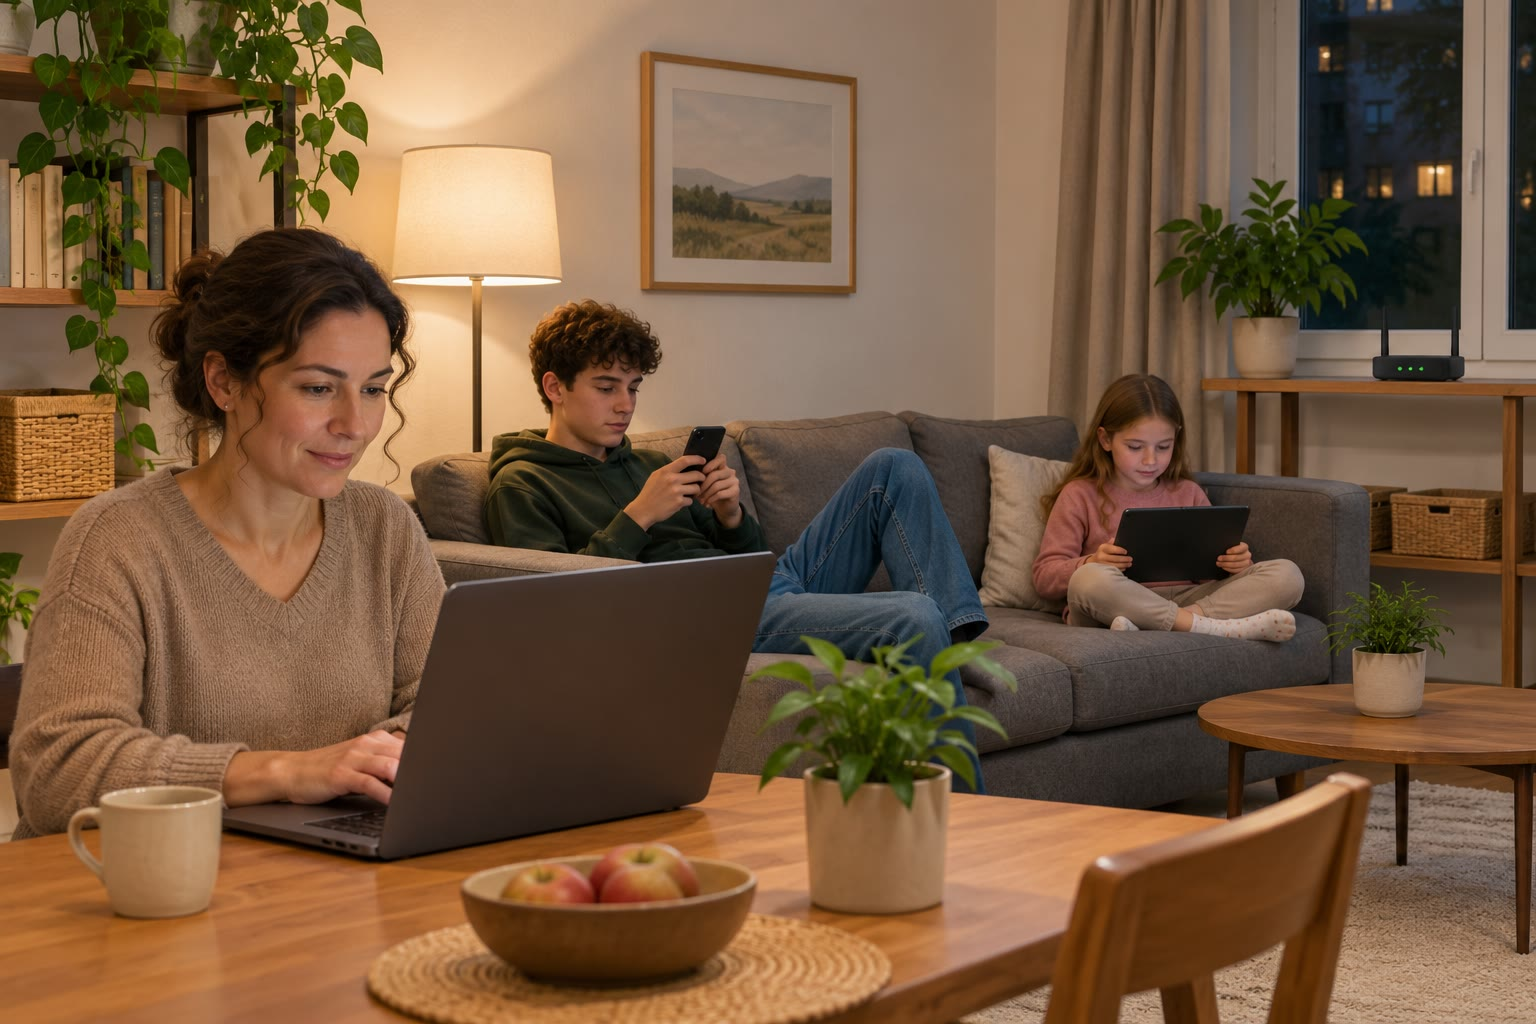
\includegraphics[width=0.55\linewidth]{images/book1/ai/g5-networks-first-look-family.jpg}

{\small A home \omterm{def:g5:networks-first-look:network}{network}: a laptop, a phone and a tablet, all linked by radio to
the small box on the shelf by the window.}
\end{omfigure}

\begin{omfigure}
\begin{tikzpicture}[x=1cm, y=1cm, font=\footnotesize,
    dev/.style={draw=black!60, fill=ocMint!25, rounded corners=2pt, minimum width=1.9cm, minimum height=0.8cm, align=center}]
  \node[draw=black!70, fill=ocYellow!40, rounded corners=3pt, minimum width=2.4cm, minimum height=0.9cm, align=center] (box) at (0,0) {home box};
  \node[dev] (lap) at (-4,1.4) {laptop};
  \node[dev] (pr) at (-4,-1.4) {printer};
  \node[dev] (tab) at (4,1.4) {tablet};
  \node[dev] (ph) at (4,-1.4) {phone};
  \node[draw=black!60, fill=ocBlue!15, cloud, cloud puffs=11, aspect=2.2, minimum width=2.6cm, minimum height=1.2cm] (net) at (0,2.7) {the Internet};
  \draw[very thick, black!70] (box) -- (lap);
  \draw[very thick, black!70] (box) -- (pr);
  \draw[very thick, black!70] (box) -- node[right] {cable to the outside} (net);
  \draw[thick, ocBlue!80!black, dashed] (box) -- (tab);
  \draw[thick, ocBlue!80!black, dashed] (box) -- (ph);
  \draw[very thick, black!70] (-6.2,-2.6) -- (-5.4,-2.6) node[right, black] {cable};
  \draw[thick, ocBlue!80!black, dashed] (-3.4,-2.6) -- (-2.6,-2.6) node[right, black] {radio (wi-fi)};
\end{tikzpicture}

{\small A home \omterm{def:g5:networks-first-look:network}{network}. Every \omterm{def:g3:inside-the-computer:device}{device} is linked to the home box, by cable
(solid lines) or by radio (dashed lines); the box \omterm{def:g5:networks-first-look:web}{links} the home to the
\omterm{def:g5:networks-first-look:internet}{Internet}.}
\label{fig:g5:networks-first-look:home}
\end{omfigure}

\section{The Internet is a network of networks}

\begin{definition}[Internet]\label{def:g5:networks-first-look:internet}
The \emph{Internet}\index{Internet} is the worldwide \omterm{def:g5:networks-first-look:network}{network} made of millions
of \omterm{def:g5:networks-first-look:network}{networks} linked to each other: home \omterm{def:g5:networks-first-look:network}{networks}, school \omterm{def:g5:networks-first-look:network}{networks}, the \omterm{def:g5:networks-first-look:network}{networks}
of companies, and the large \omterm{def:g5:networks-first-look:network}{networks} that join them across countries and
under the seas.
\end{definition}

No single \omterm{def:g1:what-is-a-computer:computer}{computer} is the \omterm{def:g5:networks-first-look:internet}{Internet}, and nobody owns all of it. Noor's photo
leaves her home \omterm{def:g5:networks-first-look:network}{network}, goes through the \omterm{def:g5:networks-first-look:network}{network} of the company that brings
the \omterm{def:g5:networks-first-look:internet}{Internet} to her street, then through large \omterm{def:g5:networks-first-look:network}{networks} that cross the
countries, then through the \omterm{def:g5:networks-first-look:network}{network} that serves her grandmother's town, and at
last into her grandmother's phone. At each step, a \omterm{def:g1:what-is-a-computer:computer}{computer} reads where the
data must go and passes it on.

\begin{omfigure}
\begin{tikzpicture}[x=1cm, y=1cm, font=\footnotesize,
    cl/.style={draw=black!60, fill=ocBlue!12, cloud, cloud puffs=10, aspect=1.8, minimum width=2.6cm, minimum height=1.4cm, align=center}]
  \node[cl] (a) at (0,0) {Noor's\\home network};
  \node[cl] (b) at (3.6,1.3) {her street's\\network};
  \node[cl] (c) at (7.4,1.3) {a network\\across countries};
  \node[cl] (d) at (11,0) {grandmother's\\town network};
  \node[cl] (e) at (5.5,-1.4) {another\\network};
  \draw[black!50, thick] (a) -- (e) (e) -- (d) (b) -- (e) (c) -- (e);
  \draw[ocRed!80!black, line width=1.6pt, -{Stealth[length=3mm]}] (a) -- (b);
  \draw[ocRed!80!black, line width=1.6pt, -{Stealth[length=3mm]}] (b) -- (c);
  \draw[ocRed!80!black, line width=1.6pt, -{Stealth[length=3mm]}] (c) -- (d);
\end{tikzpicture}

{\small The \omterm{def:g5:networks-first-look:internet}{Internet} as \omterm{def:g5:networks-first-look:network}{networks} joined to \omterm{def:g5:networks-first-look:network}{networks}. The red arrows show one
path that Noor's photo can take; the data could also go another way.}
\label{fig:g5:networks-first-look:internet}
\end{omfigure}

\section{The web}

\begin{definition}[Server]\label{def:g5:networks-first-look:server}
A \emph{server}\index{server} is a \omterm{def:g1:what-is-a-computer:computer}{computer}, linked to the \omterm{def:g5:networks-first-look:internet}{Internet}, that
keeps \omterm{def:g3:files-and-folders:file}{files} and \omterm{def:g4:programs-and-operating-system:program}{programs} and sends them to the other \omterm{def:g1:what-is-a-computer:computer}{computers} that ask for
them.
\end{definition}

\begin{definition}[Web page and browser]\label{def:g5:networks-first-look:page}
A \emph{web page}\index{web page} is a \omterm{def:g3:files-and-folders:file}{file} kept on a \omterm{def:g5:networks-first-look:server}{server}, made to be shown
on a screen: text, pictures, and \omterm{def:g5:networks-first-look:web}{links} to other pages. A
\emph{browser}\index{browser} is the \omterm{def:g4:programs-and-operating-system:application}{application} that asks a \omterm{def:g5:networks-first-look:server}{server} for a web
page and shows it.
\end{definition}

\begin{definition}[Web address]\label{def:g5:networks-first-look:address}
The \emph{web address}\index{web address} of a page tells the \omterm{def:g5:networks-first-look:page}{browser} which
\omterm{def:g5:networks-first-look:server}{server} to ask and which \omterm{def:g3:files-and-folders:file}{file} to ask for. It is typed in the address bar of the
\omterm{def:g5:networks-first-look:page}{browser}.
\end{definition}

% ledger: g5:example-domains
Take the address
\begin{center}\code{https://www.example.com/animals/cat.html}\end{center}
The part \code{www.example.com} names the \omterm{def:g5:networks-first-look:server}{server}, and \code{/animals/cat.html} is the
path of the \omterm{def:g3:files-and-folders:file}{file} on that \omterm{def:g5:networks-first-look:server}{server}, written like a path on our own \omterm{def:g1:what-is-a-computer:computer}{computer}
(\cref{ch:g3:files-and-folders}). (The name \code{example.com} is kept free
for examples like this one: it belongs to nobody.)

\begin{omfigure}
\begin{tikzpicture}[x=1cm, y=1cm, font=\footnotesize]
  \omwindow{7.2}{3.6}{Browser}
  \pic at (0,0) {window};
  \draw[black!50, fill=black!4, rounded corners=1pt] (0.2,2.65) rectangle (7.0,3.05);
  \node[anchor=west, font=\scriptsize\ttfamily] at (0.25,2.85) {https://www.example.com/animals/cat.html};
  \node[font=\small\bfseries] at (3.6,2.15) {Cats};
  \draw[black!30] (0.5,1.75) -- (5.9,1.75) (0.5,1.5) -- (5.9,1.5) (0.5,1.25) -- (4.4,1.25);
  \node[font=\scriptsize, text=ocBlue!80!black] at (1.2,0.6) {\underline{Dogs}};
  \node[font=\scriptsize, text=ocBlue!80!black] at (2.6,0.6) {\underline{Birds}};
  % server
  \draw[black!70, fill=black!15, rounded corners=2pt] (10.6,0.2) rectangle (12.2,3.4);
  \foreach \y in {0.7,1.4,2.1,2.8} {\draw[black!60, fill=black!30] (10.75,\y-0.25) rectangle (12.05,\y+0.25); \fill[ocMint] (11.85,\y) circle (0.06);}
  \node[font=\footnotesize] at (11.4,-0.2) {server \code{www.example.com}};
  \draw[-{Stealth[length=2.5mm]}, thick, ocRed!80!black] (7.4,2.6) -- node[above, align=center] {1. ``please send\\\code{/animals/cat.html}''} (10.4,2.6);
  \draw[-{Stealth[length=2.5mm]}, thick, ocBlue!80!black] (10.4,1.0) -- node[below, align=center] {2. the file of the page\\comes back} (7.4,1.0);
\end{tikzpicture}

{\small The \omterm{def:g5:networks-first-look:page}{browser} asks the \omterm{def:g5:networks-first-look:server}{server} for a page, the \omterm{def:g5:networks-first-look:server}{server} sends the \omterm{def:g3:files-and-folders:file}{file} back,
and the \omterm{def:g5:networks-first-look:page}{browser} shows it. The underlined words are \omterm{def:g5:networks-first-look:web}{links} to other pages.}
\label{fig:g5:networks-first-look:browser}
\end{omfigure}

\begin{definition}[Link and World Wide Web]\label{def:g5:networks-first-look:web}
A \emph{link}\index{link (on a web page)} is a word or a picture on a \omterm{def:g5:networks-first-look:page}{web page}
that holds the address of another page: clicking it makes the \omterm{def:g5:networks-first-look:page}{browser} ask for
that page. The \emph{World Wide Web}\index{World Wide Web} is all the \omterm{def:g5:networks-first-look:page}{web pages}
of all the \omterm{def:g5:networks-first-look:server}{servers} of the \omterm{def:g5:networks-first-look:internet}{Internet}, joined by their links.
\end{definition}

\begin{omfigure}
\begin{tikzpicture}[x=1cm, y=1cm, font=\small,
    pg/.style={draw=black!60, fill=white, minimum width=1.2cm, minimum height=1.5cm, font=\large\bfseries},
    ln/.style={-{Stealth[length=2.5mm]}, thick, ocBlue!80!black}]
  \node[pg] (A) at (0,0) {A};
  \node[pg] (B) at (3.2,1.2) {B};
  \node[pg] (C) at (3.2,-1.2) {C};
  \node[pg] (D) at (6.4,0) {D};
  \draw[ln] (A) -- (B);
  \draw[ln] (A.south east) -- (C.west);
  \draw[ln] (C.north west) to[bend right=10] (A.east);
  \draw[ln] (B.east) to[bend left=12] (D.north west);
  \draw[ln] (D.west) to[bend left=12] (B.south east);
\end{tikzpicture}

{\small Four pages and their \omterm{def:g5:networks-first-look:web}{links}. An arrow from one page to another is a \omterm{def:g5:networks-first-look:web}{link}
on the first page that leads to the second.}
\label{fig:g5:networks-first-look:links}
\end{omfigure}

\begin{history}[The web was born in a laboratory]
% ledger: g5:web-proposal, g5:web-first-server, g5:web-free
In March 1989, Tim Berners-Lee, who worked at CERN, a large physics laboratory
near Geneva, wrote a first proposal for a way of linking documents across
\omterm{def:g1:what-is-a-computer:computer}{computers}. By the end of 1990, the first web \omterm{def:g5:networks-first-look:server}{server} and the first \omterm{def:g5:networks-first-look:page}{browser} were
running at CERN, on a NeXT \omterm{def:g1:what-is-a-computer:computer}{computer}. On 30 April 1993, CERN made the web
software free for everyone to use, and the web spread across the world.
\end{history}

\begin{omfigure}
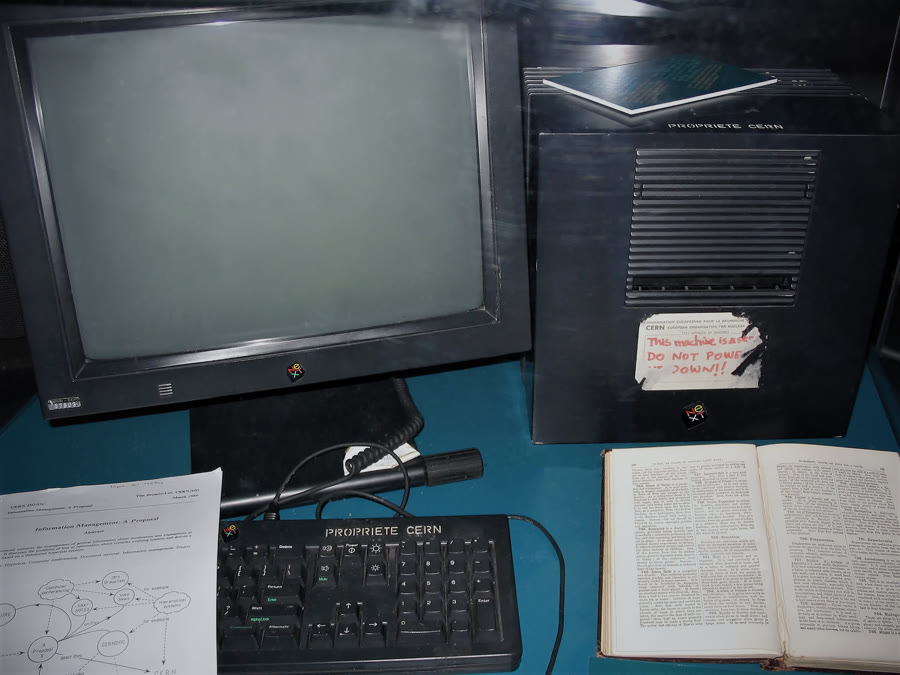
\includegraphics[width=0.45\linewidth]{images/book1/g5-first-web-server.jpg}

{\small The first web \omterm{def:g5:networks-first-look:server}{server}, a NeXT \omterm{def:g1:what-is-a-computer:computer}{computer}, kept at CERN. The paper label
asks that nobody switch it off. Photograph: Coolcaesar, CC BY-SA 3.0.}
\end{omfigure}

\section{Search engines}

How do we find a page when we do not know its address? We ask a search engine,
a website that answers a few words with a list of pages. It does not read the
whole web when we ask: that would take far too long. Long before, its \omterm{def:g4:programs-and-operating-system:program}{programs}
visited billions of pages, following their \omterm{def:g5:networks-first-look:web}{links} one after another, and noted
which words appear on which page. When we search, it looks in that list and
answers at once. The order of the answers is chosen by the search engine,
with its own rules: the first answer is not always the best one.

\begin{omfigure}
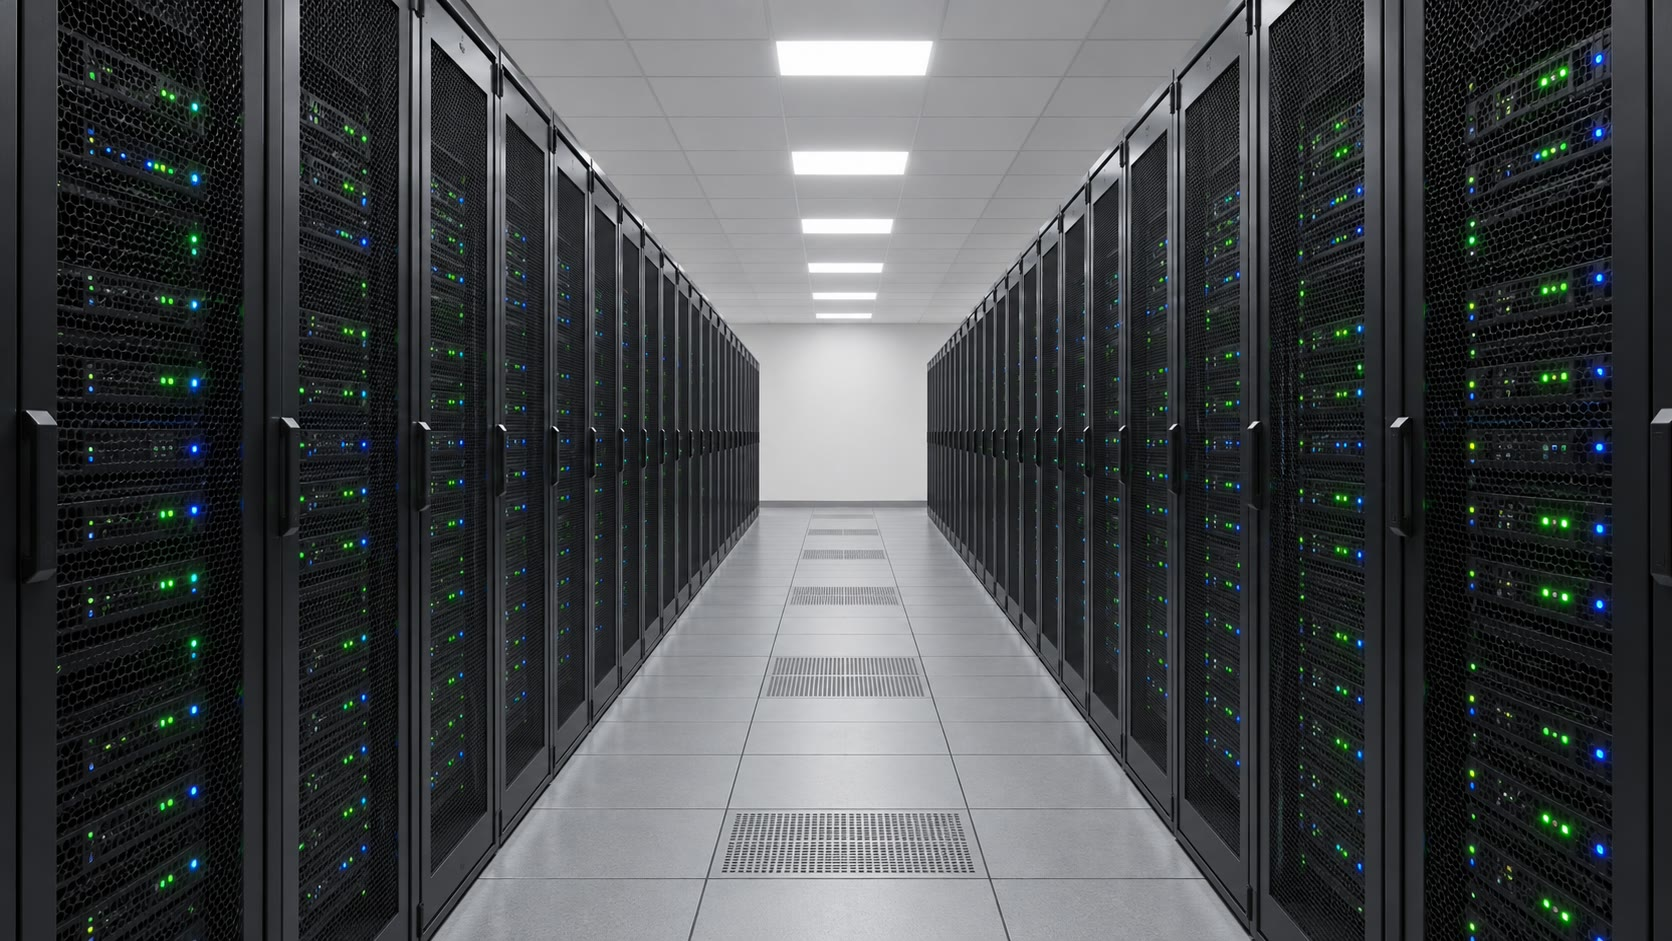
\includegraphics[width=0.55\linewidth]{images/book1/ai/g5-networks-first-look-data-centre.jpg}

{\small \omterm{def:g5:networks-first-look:server}{Servers} in a data centre: rows of cabinets, each full of \omterm{def:g1:what-is-a-computer:computer}{computers}.
Search engines and large websites run on thousands of them.}
\end{omfigure}

\section{A password is a key}

Our messages, photos and accounts are kept on \omterm{def:g5:networks-first-look:server}{servers}, which anybody on the
\omterm{def:g5:networks-first-look:internet}{Internet} can try to reach. How does a \omterm{def:g5:networks-first-look:server}{server} know that it is really Noor who
asks for Noor's photos?

\begin{definition}[Password and authentication]\label{def:g5:networks-first-look:password}
\emph{Authentication}\index{authentication} is proving to a \omterm{def:g1:what-is-a-computer:computer}{computer} who we
are. A \emph{password}\index{password} is a secret word or phrase used for it:
whoever knows the password can open the account, as whoever has the key can
open the door.
\end{definition}

A \omterm{def:g5:networks-first-look:password}{password} is strong if it is hard to guess, even by a \omterm{def:g1:what-is-a-computer:computer}{computer} that tries
millions of \omterm{def:g5:networks-first-look:password}{passwords}. Let us count. A code of 4 digits has 10 choices for the
first digit, 10 for the second, and so on: $10 \times 10 \times 10 \times 10 =
\num{10000}$ codes. A \omterm{def:g1:what-is-a-computer:computer}{computer} tries them all in a moment. A \omterm{def:g5:networks-first-look:password}{password} of 12
characters, each a small letter or a digit, has 36 choices for each character:
36 multiplied by itself, 12 times over, makes more than four billion billion
\omterm{def:g5:networks-first-look:password}{passwords}. Each extra character multiplies the number of possibilities, so a
long \omterm{def:g5:networks-first-look:password}{password} is much stronger than a short one.

\begin{safety}
% ledger: g5:passwords-guidance
Make your \omterm{def:g5:networks-first-look:password}{passwords} long: three random words put together, like
``kettle-giraffe-snowstorm'', are long, easy to remember and hard to guess.
Never use your name, your birthday or ``1234''. Use a different \omterm{def:g5:networks-first-look:password}{password} for
each important account. Never tell a \omterm{def:g5:networks-first-look:password}{password} to anyone, even a friend; only a
parent or a teacher may help you with it.
\end{safety}

\section{Exercises}

\begin{exercise}[$\star$]\label{exo:g5:networks-first-look:1}
Name three \omterm{def:g3:inside-the-computer:device}{devices} of a home \omterm{def:g5:networks-first-look:network}{network}. How is each one linked to the home box?
\end{exercise}

\begin{exercise}[$\star$]\label{exo:g5:networks-first-look:2}
Sami says: ``The \omterm{def:g5:networks-first-look:internet}{Internet} is a very big \omterm{def:g1:what-is-a-computer:computer}{computer} somewhere.'' Is he right?
\end{exercise}

\begin{exercise}[$\star$]\label{exo:g5:networks-first-look:3}
What does a \omterm{def:g5:networks-first-look:page}{browser} do?
\end{exercise}

\begin{exercise}[$\star$]\label{exo:g5:networks-first-look:4}
What does a \omterm{def:g5:networks-first-look:server}{server} keep, and what does it do with it?
\end{exercise}

\begin{exercise}[$\star$]\label{exo:g5:networks-first-look:5}
In the drawing of the four pages, find a way to go from page A to page D by
clicking \omterm{def:g5:networks-first-look:web}{links}. Can you then go from D back to A?
\end{exercise}

\begin{exercise}[$\star$]\label{exo:g5:networks-first-look:6}
Strong or weak? ``1234'', ``anna'', ``purple-tractor-moonlight'', ``qwerty'',
``Tom2015'', ``giraffe kettle snowstorm''.
\end{exercise}

\begin{exercise}[$\star$]\label{exo:g5:networks-first-look:7}
How many different codes of 3 digits are there?
\end{exercise}

\begin{exercise}[$\star$]\label{exo:g5:networks-first-look:8}
How many different \omterm{def:g5:networks-first-look:password}{passwords} of 4 small letters are there? Write the
multiplication, then compute it.
\end{exercise}

\begin{exercise}[$\star\star$]\label{exo:g5:networks-first-look:9}
Why should you use a different \omterm{def:g5:networks-first-look:password}{password} for each important account?
\end{exercise}

\begin{exercise}[$\star\star$]\label{exo:g5:networks-first-look:10}
Adding one character to a \omterm{def:g5:networks-first-look:password}{password} multiplies the number of possible
\omterm{def:g5:networks-first-look:password}{passwords}. By how much, if the characters are digits? If they are small
letters?
\end{exercise}

\begin{exercise}[$\star\star$]\label{exo:g5:networks-first-look:11}
A search engine answers in less than a second. What has it done before you
searched, so that it can answer so fast?
\end{exercise}
